%!TEX root = ../dokumentation.tex

\chapter{Umsetzung}

Ein bisschen BlaBla, dass jetzt auf die Umsetzung eingegangen wird.

%title wird unter dem Bsp. abgedruckt
%caption wird im Verzeichnis abgedruckt
%label wird zum referenzieren benutzt, muss einzigartig sein.

\section{Voraussetzungen}
Hier kommt der Scheiß ist zustand rein

Hier genau erklären was gemacht werden muss, damit man unser Programm nutzen kann(mit Code und Linux Befehlen und so)

\href{https://github.com/alexanderklapdor/RaspberryPi_Go_Audioplayer#installation}{Schritt für Schritt für die Voraussetzung}

\section{Konzept}
Hier kommt der Scheiß ist zustand rein
\begin{figure}[h]
	\centering
	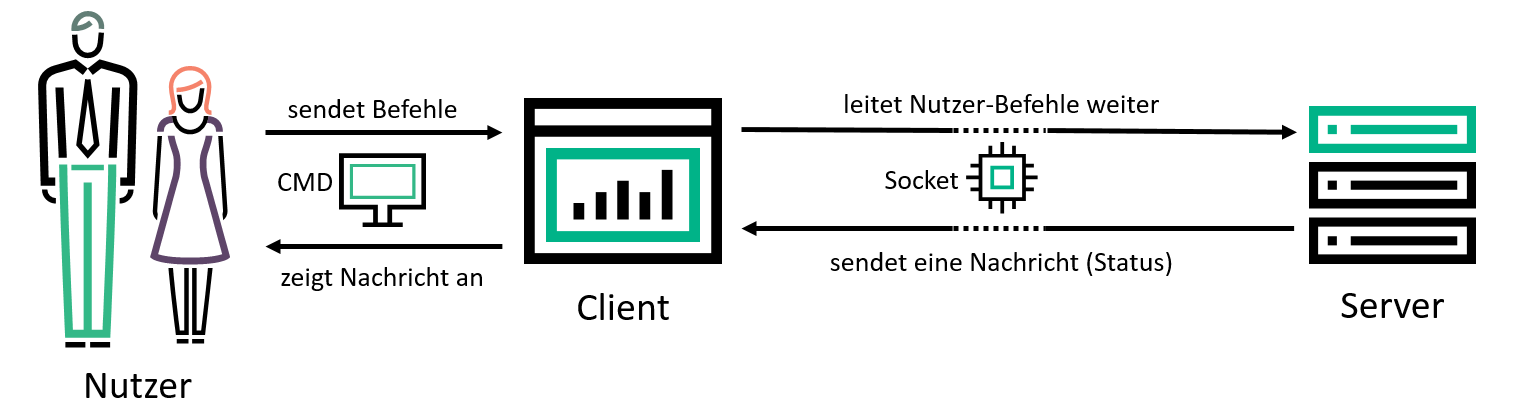
\includegraphics[scale=0.5]{Audioplayer_Konzept.png}
	\caption{Audioplayer - Konzept}
	\label{img:grafik-RaspberryPi3}
\end{figure}
\newline

\subsection{Konzept des Clients}
Hier kommt der Scheiß ist zustand rein

1. Holt sich die Config(da stehen alle Sachen drinnen wie Ort des Sockets und blabla)\\
2. Setzt den Logger auf \\
3. Überprüft ob der Server bereits läuft, wenn nicht dann startet er den Server und wartet solange bis er hochgefahren ist und die Verbindung zum socket besteht. \\
4. Überprüft ob Übergabeparameter(Kommando) übergeben wurden. Wenn nicht dann Programm beenden, wenn doch dann Parsen den Übergabewerte \\
5. Packen der geparsten Informationen in ein JSON Format und senden dies JSON über den Socket an den Server. \\
6. Beenden des Clients \\

\subsection{Konzept des Servers}

1. Holt sich die Config(da stehen alle Sachen drinnen wie Ort des Sockets und blabla)\\
2. Setzt den Logger auf \\
3. Setzt den Socket auf \\
4. Starten Pulseaudio \\
5. Hört den Socket ab \\
	5.1 Falls nichts kommt...warten \\
	5.2 Falls was reinkommt - JSON Parsen und das gewünschte Kommando ausführen.\\
	

\section{Kommunikation über Sockets}
Sockets erklären und kurz erläutern warum wir die verwendet haben.\\
\\
Ein Socket (von engl. Sockel, Steckverbindung oder Steckdose) ist ein vom Betriebssystem bereitgestelltes Objekt, das als Kommunikationsendpunkt dient. Ein Programm verwendet Sockets, um Daten mit anderen Programmen auszutauschen. Das andere Programm kann sich dabei auf demselben Computer (Interprozesskommunikation) oder einem anderen, via Netzwerk erreichbaren Computer befinden. Die Kommunikation über Sockets erfolgt in der Regel bidirektional, das heißt, über das Socket können Daten sowohl empfangen als auch gesendet werden.

\section{Funktionen des Programms}
Hier kommen die Scheiß Funktionen rein, alle Beschreiben und vll. kurz erläutern evtl. an einer Zeichnung wie diese Ablaufen.

\href{https://github.com/alexanderklapdor/RaspberryPi_Go_Audioplayer#commands-of-the-client}{Kommandos}
\\
\href{https://github.com/alexanderklapdor/RaspberryPi_Go_Audioplayer#console-arguments}{Console-Arguments}


\section{Bedienung des Programms}
Beispiele für die Bedienung reinmachen ( Ordner abspielen, Loop, Playlist, blabla)

